\documentclass{standalone}
\usepackage{tikz}
\begin{document}
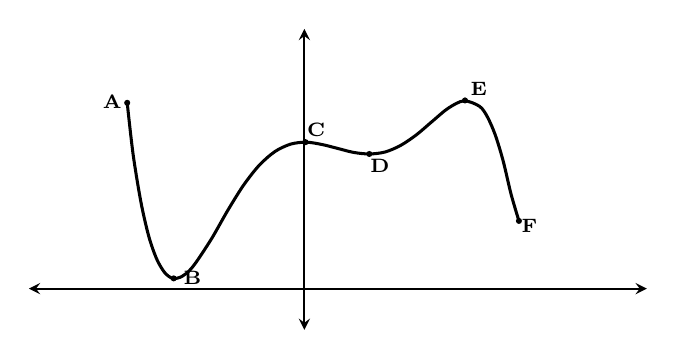
\begin{tikzpicture}[color=black, >=stealth, scale=0.5, font=\scriptsize\bfseries]
  % Axes (no scale shown on the original figure)
  \draw[<->, thick] (-7.0,0) -- (8.7,0);
  \draw[<->, thick] (0,-1.05) -- (0,6.6);
  % Graph of f
  \draw[line width=1.1pt, smooth] plot coordinates {
    (-4.50,4.72) (-4.35,3.41) (-4.15,2.19) (-3.95,1.32) (-3.75,0.75)
    (-3.55,0.41) (-3.35,0.26) (-3.15,0.29) (-2.95,0.43) (-2.75,0.67)
    (-2.35,1.28) (-1.95,1.98) (-1.55,2.62) (-1.15,3.13) (-0.75,3.48)
    (-0.35,3.67) (0.05,3.72) (0.45,3.66) (0.85,3.56) (1.25,3.46)
    (1.65,3.42) (2.05,3.47) (2.45,3.64) (2.85,3.91) (3.25,4.25)
    (3.65,4.58) (4.05,4.77) (4.45,4.63) (4.65,4.36) (4.85,3.90)
    (5.05,3.24) (5.25,2.40) (5.45,1.72)
  };
  % The six labeled points
  \fill (-4.50,4.72) circle (2.2pt) ;
  \fill (-3.32,0.26) circle (2.2pt);
  \fill (0.03,3.72) circle (2.2pt);
  \fill (1.65,3.42) circle (2.2pt);
  \fill (4.08,4.78) circle (2.2pt);
  \fill (5.45,1.72) circle (2.2pt);
  \node at (-4.88,4.75) {A};
  \node at (-2.84,0.27) {B};
  \node at (0.30,4.03) {C};
  \node at (1.92,3.13) {D};
  \node at (4.43,5.07) {E};
  \node at (5.72,1.60) {F};
\end{tikzpicture}
\end{document}
